%
% Einfache LaTeX-Vorlage f�r Arbeiten am Lehrstuhl Kranzlm�ller / MNM-Team
% - optimiert f�r die Arbeit mit g�ngigen LaTeX-Editoren
% - funktioniert ohne Makefile und Anpassungen der LaTeX-Verzeichnisstruktur
% - verwendet Komaskript f�r ein (nach europ�ischen Gepflogenheiten) sch�neres Layout
% 
% v1, 2007 (Michael Brenner)
% Diese Version: v1.1, 2012 (Michael Brenner)
% Diese Version: v1.2, 2017 (Michael Brenner)
% 


\documentclass[bibliography=totoc,listof=totoc,BCOR=5mm,DIV=12]{scrbook} % Rand f�r Bindung: 5mm / falls Index verwendet, erg�nze "index=totoc" zu den Optionen 
\usepackage{ngerman} % Trennung nach neuer deutscher Rechtschreibung, deutsche Sonderzeichen, z.B. \glqq und \grqq f�r deutsche Anf�hrungszeichen 
\usepackage[latin1]{inputenc} % Umlaute im Text
\usepackage{graphicx} % Einf�gen von Grafiken  - f�r PDF-Latex: .pdf und .png (.jpg m�glich, sollte aber vermieden werden)
\usepackage{url}           % URL's (z.B. in Literatur) sch�ner formatieren
\usepackage{hyperref} % sorgt f�r f�r Hyperlinks in PDF-Dokumenten

\graphicspath{{./Bilder/}}

%
% der Befehl \hypenation versteht keine Sonderzeichen, also weder �
% noch "a noch \"a. W�rter die derartige Zeichen enthalten m�ssen
% direkt im Text getrennt werden, z.B. W�r\-ter
%
\hyphenation{Ma-nage-ment}
\hyphenation{Ma-nage-ment-agent}
\hyphenation{Ma-nage-ment-agent-en}
\hyphenation{Ma-nage-ment-ar-chi-tek-tur}
\hyphenation{Ma-nage-ment-ar-chi-tek-tu-ren}
\hyphenation{Ma-nage-ment-an-wen-dung}
\hyphenation{Ma-nage-ment-an-wen-dung-en}
\hyphenation{Ma-nage-ment-an-for-der-ung}
\hyphenation{Ma-nage-ment-funk-ti-on}
\hyphenation{Ma-nage-ment-funk-ti-onen}
\hyphenation{Ma-nage-ment-kon-zep-te}
\hyphenation{Ma-nage-ment-res-source}
\hyphenation{Ma-nage-ment-in-for-ma-ti-on}
\hyphenation{Ma-nage-ment-res-sour-cen}
\hyphenation{ma-nage-ment-re-le-vante}
\hyphenation{ma-nage-ment-sy-stem}
\hyphenation{ma-nage-ment-sy-steme}
\hyphenation{Ma-nage-ment-in-stru-men-tie-rung}
\hyphenation{Ma-nage-ment-platt-form}
\hyphenation{Sys-te-men}
\hyphenation{Sys-tem-um-ge-bun-gen}
\hyphenation{Sys-tem-ma-nage-ment}
\hyphenation{DHCP}
\hyphenation{Ma-nage-ment-diszi-plinen}
\hyphenation{System-management-architekturen}
\hyphenation{Verwendungs-nachweise}
\hyphenation{Video-einricht-ungen}
\hyphenation{Res-source}
\hyphenation{Res-sourcen}
\hyphenation{Grund-anwendung}
\hyphenation{Grund-anwendungen}
\hyphenation{Basis-anwendung}
\hyphenation{Core}
\hyphenation{Kom-mu-ni-ka-ti-on}
\hyphenation{De-sign-ent-schei-dung}
\hyphenation{Sprung-ad-res-sen}
\hyphenation{Klas-si-fi-ka-ti-on}
\hyphenation{Schreib-recht}
\hyphenation{Be-nut-zer-zer-ti-fi-kat}
\hyphenation{Bau-stein-ent-wi-ckler}
\hyphenation{ad-mi-ni-stra-ti-ve}

 % in dieses File kommen W�rter die Latex nicht richtig trennt

\begin{document}

% ---------------------------------------------------------------
\frontmatter % Titelbl�tter und Erkl�rung jeweils spezifisch f�r die jeweilige Uni einbinden
    %%%%%%%%%%%%%%%%%%%%%%%%%%%%%%%
% erste Seite

\thispagestyle{empty}

\begin{center}

\vspace*{-2cm}

{\Huge INSTITUT F�R INFORMATIK\\[1mm]}
DER LUDWIG--MAXIMILIANS--UNIVERSIT�T M�NCHEN\\

\vspace*{1cm}


\includegraphics[width=0.3\textwidth]{lmu_siegel}

\vspace*{2cm}

{\Large \textbf{Master's Thesis}}\\ % oder Fortgeschrittenenpraktikum, Master's Thesis, Bachelorarbeit etc.

\vspace{2.0cm}
{\Huge \textbf{C++ Graph Concepts for}}\\
\vspace*{3mm}
{\Huge \textbf{Partitioned Global Address Space}}\\
\vspace*{20mm}

{\LARGE Stefan Effenberger} % Name des Autors

\vspace{3cm}
\end{center}

\newpage

%%%%%%%%%%%%%%%%%%%%%%%%%%%%%%%
% zweite Seite

\thispagestyle{empty}
\cleardoublepage

%%%%%%%%%%%%%%%%%%%%%%%%%%%%%%%
% dritte Seite (Kopie der ersten)

\thispagestyle{empty}

\begin{center}

\vspace*{-2cm}

{\Huge INSTITUT F�R INFORMATIK\\[1mm]}
DER LUDWIG--MAXIMILIANS--UNIVERSIT�T M�NCHEN\\

\vspace*{1cm}


\includegraphics[width=0.3\textwidth]{lmu_siegel}

\vspace*{2cm}

{\Large \textbf{Master's Thesis}}\\ % oder Fortgeschrittenenpraktikum, SEP etc.

\vspace{2.0cm}
{\Huge \textbf{C++ Graph Concepts for}}\\
\vspace*{3mm}
{\Huge \textbf{Partitioned Global Address Space}}\\
\vspace*{20mm}

{\LARGE Stefan Effenberger} % Name des Autors
\vspace{2cm}

\parbox{1cm}{
\begin{large}
\begin{tabbing}
Aufgabensteller: \hspace{.5cm} \=Prof. Dr. Dieter Kranzlm�ller\\[2mm]
Betreuer:
\>Tobias Fuchs\\[5mm]
Abgabetermin: \> \textcolor{red}{ADD DATE}\\
\end{tabbing}
\end{large}}\\
\vspace{5mm}

\end{center}
 % Titelbl�tter LMU - auskommentieren falls TUM-Arbeit
%    % Richtlinien, siehe http://wwwpa.in.tum.de/generell/Abschlussarbeitsform.html
%
%%%%%%%%%%%%%%%%%%%%%%%%%%%%%%%


% Deckblatt

\thispagestyle{empty}

\begin{center}
    
\includegraphics[width=3cm]{tum-logo}\\
    \vspace{.5cm}
% "Technische Universit�t M�nchen" oder alternativ das Logo der TUM
    {\Large \sc Technische Universit�t M�nchen}\\

    \vspace{1cm}
% "Fakult�t f�r Informatik"
    {\Huge \sc Fakult�t f�r Informatik\\[1mm]}


    \vspace{2cm}
% Diplomarbeit | Master's Thesis | Bachelorarbeit in Informatik | Wirtschaftsinformatik |
    {\Large \textbf{Masterarbeit in Informatik}}\\
% Thema bzw. Titel der Arbeit  (In der Sprache, in der die Arbeit verfasst wurde)
    \vspace{2.0cm}
    {\Huge \textbf{Ein Lorem-Rahmenwerk}}\\ % bei langen Titeln ggf. Schriftgr��e auf \huge herunter setzen
    \vspace*{3mm}
    {\Huge \textbf{f�r Ipsum-Systeme}}\\
    \vspace*{3mm}
    {\Huge \textbf{-- ein Dolor-Ansatz}}\\
    \vspace{1.5cm}
% Vorname und Nachname des Bearbeiters/ der Bearbeiterin
    Vorname Nachname

    \vspace{5cm} % ggf. je nach Zeilenzahl und Schriftgr��e des Titels anpassen
    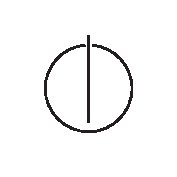
\includegraphics[width=2.4cm]{tum-info-logo}
\end{center}

\newpage

%%%%%%%%%%%%%%%%%%%%%%%%%%%%%%%
% R�ckseite Deckblatt

\thispagestyle{empty}
\cleardoublepage

%%%%%%%%%%%%%%%%%%%%%%%%%%%%%%%
% Erste Seite (Titelblatt)

\thispagestyle{empty}

\begin{center}

    
\includegraphics[width=3cm]{tum-logo}\\
    \vspace{.5cm}
    {\Large \sc Technische Universit�t M�nchen}\\


    \vspace{.5cm}

    {\huge \sc Fakult�t f�r Informatik\\[1mm]}


    \vspace{1cm}

    {\Large \textbf{Diplomarbeit in Informatik}}\\ % oder SEP etc.

% Thema bzw. Titel der Arbeit  (In der Sprache, in der die Arbeit verfasst wurde)
    \vspace{1.5cm}
    {\huge \textbf{Ein Lorem-Rahmenwerk}}\\ % bei langen Titeln ggf. Schriftgr��e herunter setzen
    \vspace*{3mm}
    {\huge \textbf{f�r Ipsum-Systeme}}\\
    \vspace*{3mm}
    {\huge \textbf{-- ein Dolor-Ansatz}}\\

% die englische bzw. deutsche Entsprechung des Titels
    \vspace{1cm}
    {\huge \textbf{A Lorem Framework}}\\ % bei langen Titeln ggf. Schriftgr��e herunter setzen
    \vspace*{3mm}
    {\huge \textbf{for Ipsum Systems}}\\
    \vspace*{3mm}
    {\huge \textbf{-- a Dolor Approach}}\\
    \vspace{1cm}

    \parbox{1cm}{
      \begin{large}
        \begin{tabbing}
          Bearbeiter: \hspace{1.5cm}
            \=Vorname Nachname\\[2mm]
    Aufgabensteller: \>Prof. Dr. Dieter Kranzlm�ller\\[2mm]
    Betreuer: \>MNM-Team-Betreuer 1\\ % alphabetische Reihenfolge (Nachname)
    \>MNM-Team-Betreuer 2\\
    \>Externer Betreuer 1 (Firma)\\[5mm]
    Abgabedatum: \> 7. Juli 2077\\
        \end{tabbing}
      \end{large}
    }\\

    \vspace{.3cm}

    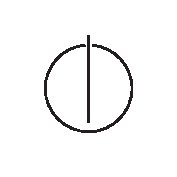
\includegraphics[width=2.4cm]{tum-info-logo}

\end{center}
 % Titelbl�tter TUM - auskommentiert lassen falls LMU-Arbeit
    \thispagestyle{empty}
    \cleardoublepage
    %
% LaTeX-Rahmen f�r Arbeiten am Lehrstuhl Hegering
%
% Harald Roelle, 2001, 2002
%
% basierend auf Arbeiten von Helmut Reiser, Boris Gruschke und Stephen Heilbronner
%

\newpage

\thispagestyle{empty}

\begin{large}

\vspace*{2cm}

\noindent
Hiermit versichere ich, dass ich die vorliegende Masterarbeit
selbst�ndig verfasst und keine anderen als die angegebenen Quellen
und Hilfsmittel verwendet habe.

\vspace{2cm}

\noindent
M�nchen, den \textcolor{red}{ADD DATE}

\vspace{3cm}

\hspace*{7cm}%
\dotfill\\
\hspace*{8.5cm}%
\textit{(Unterschrift des Kandidaten)}

\end{large}
 % Erkl�rung (Arbeit selbstst�ndig verfasst) - auskommentieren falls TUM-Arbeit
%    \begin{large}

\vspace*{2cm}
\noindent
Ich versichere, dass ich diese Masterarbeit % (bzw. Master's Thesis)
selbst�ndig verfasst und nur die angegebenen Quellen und Hilfsmittel verwendet habe.

\vspace{2cm}

\noindent
M�nchen, den 7. Juli 2077

\vspace{3cm}

\hspace*{7cm}%
\dotfill\\
\hspace*{8.5cm}%
\textit{(Unterschrift des Kandidaten)}

\end{large}
 % Erkl�rung (Arbeit selbstst�ndig verfasst) - auskommentiert lassen falls LMU-Arbeit
    \thispagestyle{empty}
    \cleardoublepage
    \vspace*{2cm}

\begin{center}
    \textbf{Abstract}
\end{center}

\vspace*{1cm}

\noindent Hier steht eine kurze Zusammenfassung der Arbeit. Sie darf auf gar keinen Fall
l�nger als eine Seite sein, ca. eine drittel bis eine halbe Seite ist optimal.

 % Abstract
    \thispagestyle{empty}
    \tableofcontents % Inhaltsverzeichnis

% ---------------------------------------------------------------
\mainmatter % die eigentliche Arbeit

    \chapter{Finibus Bonorum et Malorum}

Lorem ipsum dolor sit amet, consectetuer adipiscing elit. Nullam et lectus ac lacus bibendum ullamcorper. Sed ante neque, scelerisque eu, sodales quis, elementum nec, risus. Aliquam erat volutpat. Suspendisse potenti. Praesent erat justo, viverra sed, dignissim ut, tempus eget, orci. Morbi luctus ultrices tortor. Maecenas sit amet enim. Morbi facilisis fringilla nunc. Fusce venenatis nunc a nunc. Quisque interdum pretium erat. In mattis feugiat sapien. Aliquam erat volutpat. Proin pellentesque ullamcorper risus. Integer at risus ut velit eleifend sagittis.

\section{In adipiscing purus et purus}

\glqq Vestibulum eu\grqq\ velit \cite{praxisbuch2017} (Zitat aus einem Buch). Donec pharetra feugiat elit. Morbi vitae arcu. Sed dignissim, lectus at ultricies fringilla, mauris mi eleifend mi, nec varius ipsum nunc a enim. Vivamus quis libero a erat varius accumsan. Nullam porttitor, est vitae dignissim eleifend, lacus mi semper justo, elementum imperdiet ante nibh sed nisl. Pellentesque suscipit venenatis ipsum. Suspendisse ultricies elit et neque. Sed risus erat, vehicula eget, vulputate sit amet, viverra sit amet, arcu. Integer malesuada risus vitae est. Donec vulputate, enim a laoreet vehicula, est magna vulputate justo, ut congue sapien mi gravida arcu. Curabitur luctus sapien id orci. Maecenas pulvinar, dolor id placerat convallis, mi metus fringilla enim, eu dignissim urna justo sollicitudin nibh. Vestibulum tellus nisi, nonummy vitae, aliquet a, vehicula et, justo.

Donec viverra tortor non lectus. Vestibulum vel nulla ac sapien tristique imperdiet. Sed neque. Suspendisse porta risus nec mi. Nulla id orci. Donec nunc dolor, ullamcorper sit amet, imperdiet vitae, blandit et, lacus. Cum sociis natoque penatibus et magnis dis parturient montes, nascetur ridiculus mus. Suspendisse potenti. Ut nibh. Cras enim. Mauris a ligula scelerisque ligula dictum cursus. Proin malesuada massa non nulla. Praesent imperdiet massa eu justo.

%Grafik aus PNG-File - bei dieser Variante darauf achten, dass die Grafik in ausreichender Aufl�sung vorliegt (so dass auch nach Skalierung >300dpi im Ausdruck erreicht werden) 
\begin{figure}[htb]
  \centering
  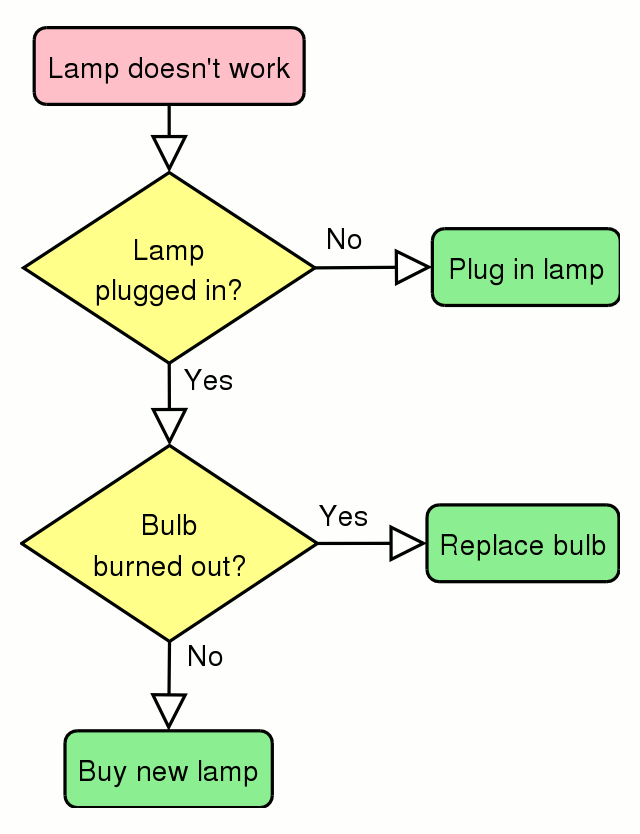
\includegraphics[width=.4\textwidth]{LampFlowchart}\\ % PNG-File
  \caption{Nulla interdum aliquam leo}\label{fig:LampFlowchart}
\end{figure}


Vestibulum ante ipsum primis in faucibus orci luctus et ultrices posuere cubilia Curae (vgl. Abbildung \ref{fig:LampFlowchart}); Curabitur mauris urna, tincidunt eget, porttitor in, lacinia vel, massa. Integer nonummy, elit at ullamcorper facilisis, massa sem elementum sapien, non malesuada ipsum lacus sed enim. Cras nec eros ut sapien sodales scelerisque. Sed quam. Suspendisse potenti. Nunc eu tortor. Nam nisi arcu, mattis ut, vehicula et, tristique in, erat. Class aptent taciti sociosqu ad litora torquent per conubia nostra, per inceptos hymenaeos. Nullam justo. Integer eget erat at mauris tristique ultrices. Sed ullamcorper vulputate velit. Vivamus blandit erat non erat luctus venenatis. Mauris elementum semper nunc. Cras pellentesque tristique nulla. Pellentesque metus. Mauris semper mi quis pede. Proin vel tellus.

Maecenas euismod, orci in mollis scelerisque, turpis elit lobortis nunc, a venenatis nisl orci quis nibh. Duis tincidunt dictum elit. Nulla sodales est nec nisi. Phasellus consectetuer suscipit urna. Nulla augue. Pellentesque tincidunt pellentesque diam. Etiam iaculis. Cras aliquet metus sed est. Cras egestas, nibh nec commodo suscipit, mauris dolor blandit dolor, id egestas lorem nibh eu nisl. Sed tempor tempor lorem. Donec fringilla luctus quam. Nam metus magna, varius non, tempor eget, rutrum quis, velit. Maecenas sit amet neque id tellus venenatis scelerisque. Donec sed purus. Quisque eu quam a augue consequat consequat.

\section{Etiam blandit molestie ligula}

Proin pharetra ultrices enim. Maecenas dui. Mauris est eros, posuere vitae, sagittis quis, tempus ut, mauris. Fusce congue, augue imperdiet tincidunt volutpat, justo metus tristique lacus, eu ultrices mauris mi ac tellus. Praesent porttitor accumsan erat. Quisque lacinia mollis turpis. Suspendisse potenti. Morbi eu urna vel purus congue accumsan. Aliquam consectetuer nulla nec augue. Nam fringilla nisi nec felis. Donec nibh tellus, consequat quis, cursus sed, vulputate eu, orci. Donec vulputate, elit vel iaculis hendrerit, augue augue congue erat, vel vestibulum tortor dui a diam (vgl. Abbildung \ref{fig:BurgerFlowchart}). Etiam vel lorem a libero feugiat feugiat. In blandit est a est. Nulla interdum pharetra nulla. Nullam eu ipsum.

%Grafik aus PDF-File - diese Variante ist vorzuziehen, da sie die Einbundung echter Vektorgrafiken erm�glicht 
\begin{figure}[htb]
  \centering
  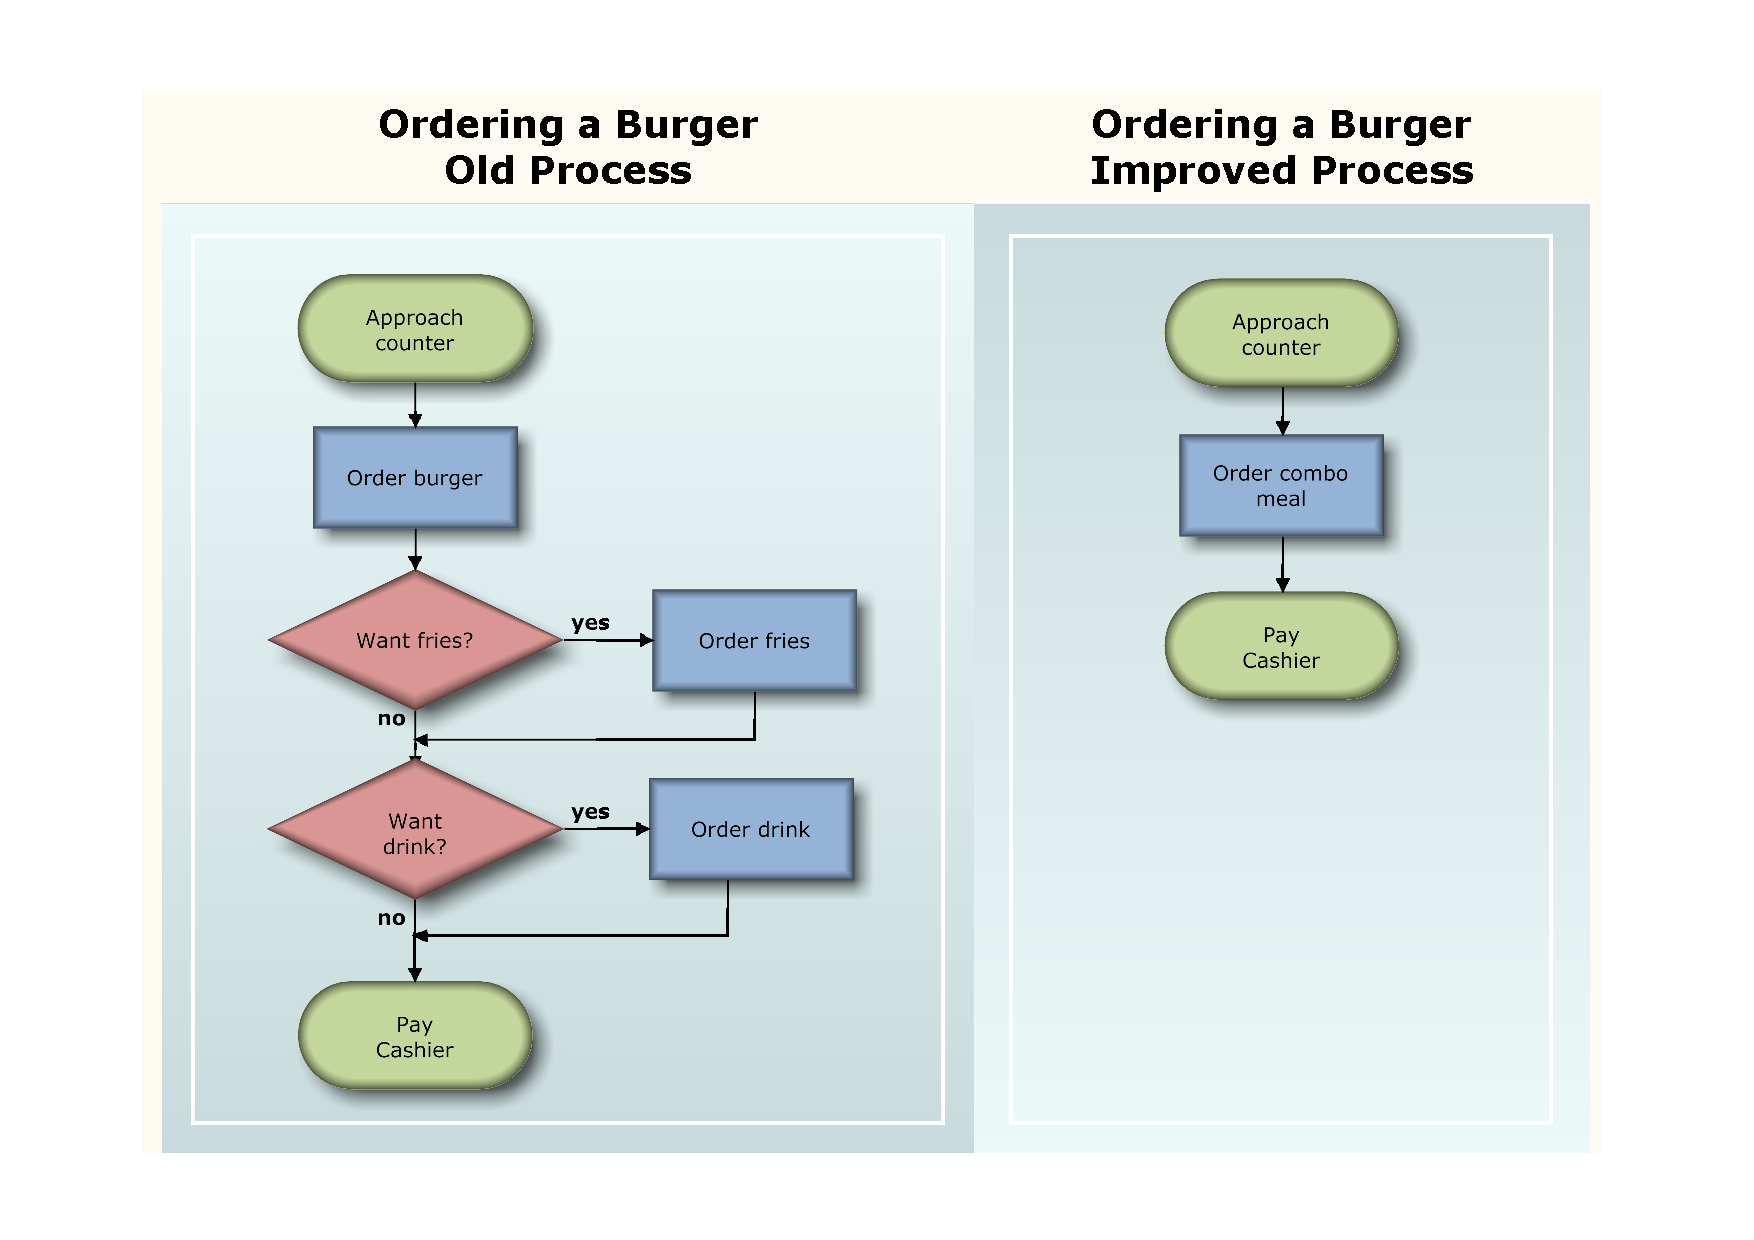
\includegraphics[scale=.6]{BurgerFlowchart}\\ % PDF-File
  \caption{Donec tempor leo a massa \cite{fitsm-0} (Zitat aus Norm, Handbuch u.�.)}\label{fig:BurgerFlowchart}
\end{figure}

Quisque ligula orci, accumsan vel, molestie ac, lacinia non, lorem . Fusce nonummy. Cras mattis, elit ac tempor congue, ante arcu porta justo, at rhoncus sapien erat vel dui \cite{latexbib}. Phasellus vestibulum, turpis non tempor vehicula, quam lacus accumsan dolor, id dictum magna magna eu neque. Sed suscipit placerat odio. Sed et sem. Mauris vel tortor a nisl egestas vulputate. Aliquam facilisis luctus nibh. Maecenas vel lectus sed urna viverra pretium. Aenean malesuada nibh sed ipsum. Fusce vel augue. Mauris eget massa. Class aptent taciti sociosqu ad litora torquent per conubia nostra, per inceptos hymenaeos. Etiam nec justo eu purus ultricies mattis. In leo ante, adipiscing sit amet, ultrices at, ultrices et, nulla. Mauris quis odio. Donec sollicitudin rutrum sapien. Aliquam eget ante a dui euismod porttitor. Donec commodo scelerisque purus. Sed magna.

Cras gravida. Praesent posuere lacus ut tellus. Nunc tempor dapibus urna. Proin sit amet velit ut urna lobortis ultrices. Suspendisse potenti. Maecenas est libero, condimentum in, mattis a, viverra in, sem. Sed nec pede. Fusce risus magna, porta eu, rhoncus vel, facilisis at, risus. Donec commodo viverra neque. Donec ultrices neque vitae justo. Nulla et magna. In condimentum tellus vitae erat. Quisque nec odio.


Nullam consectetuer risus vitae orci. Aliquam fermentum leo sit amet nulla laoreet hendrerit. Maecenas tempus, neque eu posuere vestibulum, pede eros adipiscing augue, pulvinar ullamcorper lectus lectus et tellus. Donec at velit at velit pellentesque sagittis. Vestibulum ultricies ultrices mi. Vestibulum accumsan dictum ligula. Ut lobortis, odio ut semper vehicula, nibh quam semper nisi, sed adipiscing purus lectus et sem. Mauris nisl est, scelerisque ut, ultrices nec, faucibus vitae, nulla. Nulla nisi. Suspendisse potenti. Etiam ultrices commodo odio. Quisque turpis purus, mollis sed, pretium quis, volutpat et, neque. Nam a sapien eget neque consectetuer ornare. Pellentesque felis metus, pellentesque quis, volutpat rhoncus, laoreet id, nunc. Duis egestas, felis et luctus vestibulum, velit nunc luctus felis, non tempor justo ligula et nulla. Vestibulum, Abbildung \ref{fig:tabelle}, est. Nulla aliquam eleifend justo.

%Tabellen im Regelfall auch in eine Figure-Umgebung setzen - Verwendung von Table-Umgebung lohnt nur bei sehr vielen Tabellen
\begin{figure}[htb]
  \centering
  \begin{tabular}{|l|c|}
    \hline
    \textbf{tempus} & \textbf{risus} \\ \hline
    ultrices & pellentesque \\
    rhoncus & egestas \\
    \hline
  \end{tabular}
  \caption{Aliquam fermentum}\label{fig:tabelle}
\end{figure}

Class aptent taciti sociosqu ad litora torquent per conubia nostra, per inceptos hymenaeos. Lorem ipsum dolor sit amet, consectetuer adipiscing elit. Sed auctor urna quis turpis. Suspendisse potenti. Donec tempus gravida ante. Nulla magna velit, condimentum et, pharetra sollicitudin, tincidunt et, nibh. Donec tincidunt, leo a facilisis consectetuer, quam diam cursus nibh, vitae porttitor lacus dolor in lacus. Nulla id nulla in dolor adipiscing posuere. Proin sagittis mattis dui. Maecenas neque arcu, ornare a, gravida et, posuere ut, massa. Donec congue odio ac enim. Nam malesuada sapien sit amet ante. Donec ullamcorper pulvinar dolor. Fusce posuere tellus.

\section{Ut venenatis mi id orci}

Class aptent taciti sociosqu ad litora torquent per conubia nostra, per inceptos hymenaeos. Ut quam odio, luctus gravida, aliquam eu, fringilla a, nulla. Nulla facilisi. Aliquam tincidunt porta urna. Nulla facilisi. Cras pellentesque cursus risus. Quisque semper imperdiet ante. Donec erat magna, sagittis vitae, convallis ut, tincidunt et, lectus. Mauris vulputate tincidunt mi. Integer diam enim, mollis non, dignissim non, faucibus eu, enim. Aliquam erat volutpat. Sed facilisis sagittis massa. Vivamus vel neque. Donec eu mi. Aenean lobortis. Nullam pulvinar. Mauris vel lorem vel dolor semper volutpat. Nam posuere blandit arcu.

\endinput 
%    \input{kapitel2}

% ---------------------------------------------------------------
\backmatter % ab hier keine Nummerierung mehr
    \listoffigures
    \bibliographystyle{alphadin}
    \bibliography{./Bib/stud77}

\end{document}
